


\chapter{الدراسة المرجعية}
يبيّن هذا الفصل الدراسة المرجعية للمشروع.
يبدأ بتقديم مفاهيم تعلّم الآلة ومراحلها المختلفة والمعايير المعتمدة لتقييمها.
ويقدّم مفاهيم ومراحل معالجة اللغات الطبيعية.
وأخيراً يسرد بعض الأوراق الأبحاث العلمية المتعلقة بهذا المشروع، ويوضح المنهجيات المتبعة فيها.







\section{تعلم الآلة}
\label{sec:ml}
تعلم الآلة \textenglish{Machine Learning} هو فرع جزئي من الذكاء الصنعي \textenglish{Artificial Intelligence}.
يُقصد بتعلم الآلة مجموعة الأدوات والمفاهيم والمنهجيات المستخدمة لبرمجة الحواسيب
بطريقة تسمح لهذه الحواسيب بالتعلم من المعطيات~\cite{hands-on}.

ويمكن أيضاً تعريفه بشكل أكثر عمومية كالتالي:

\begin{english}
	``Machine Learning is the field of study that gives computers the ability to learn
	without being explicitly programmed.'' \\
	--Arthur Samuel, 1959
\end{english}

كما يعتبر التعريف التالي تقني وأكثر دقة:

\begin{english}
	``A computer program is said to learn from experience $E$ with respect to some task $T$
	and some performance measure $P$, if its performance on $T$, as measured by $P$, improves
	with experience $E$.'' \\
	--Tom Mitchell, 1997
\end{english}

على سبيل المثال، النظام الذي يقوم بفلترة الإيميلات إلى إيميلات مؤذية \textenglish{spam} وإيميلات غير مؤذية \textenglish{non-spam}، يستخدم منهجيات تعلم الآلة.
يقوم هذا النظام بتعلم طريقة التمييز بين هذين النوعين من الإيميلات باستخدام عدد كبير من الأمثلة والمعطيات المصنفة مسبقاً.
نسمي هذه المجموعة من الأمثلة بمجموعة التدريب \textenglish{Training Set}، وكل مثال منها نسميه مثال تدريب \textenglish{Training Instance}.

في هذه الحالة، المهمة $T$ هي تصنيف الإيميلات الجديدة إلى إيميلات مؤذية وإيميلات غير مؤذية، الخبرة $E$ هي مجموعة مجموعة التدريب،
ومؤشر قياس الأداء $P$ يمكن تعريفه بعدّة طرق؛ فمثلاً يمكننا استخدام نسبة نسبة عدد الإيميلات التي تم تصنيفها بشكل صحيح إلى عدد الإيميلات الكلي
(هذا المعيار يسمى الصِحَّة \textenglish{Accuracy} كم سنرى لاحقاً).

\subsection{المنهجيات العامة لتعلم الآلة}
\label{sec:ml:classification}
يمكن تصنيف أنظمة تعلم الآلة وفق عدّة معايير. التصنيف الأكثر شهرة يعتمد على آلية التدريب، وهو كالتالي:
\begin{itemize}
	\item
	التعلم المشرف عليه \textenglish{Supervised Learning}:
	وهي حالة أن تكون الأمثلة التدريبية متوفرة مع الخرج \textenglish{label} المرتبط بها. وهذه حالة مثال تصنيف الإيميلات المطروح سابقاً.
	حيث أن مجموعة التدريب هي مجموعة كبيرة من الإيميلات المصنفة مسبقاً من قبل البشر إلى إيميلات مؤذية وإيميلات غير مؤذية.
	\item
	التعلم غير المشرف عليه \textenglish{Unsupervised Learning}:
	وهي حالة أن تكون مجموعة التدريب موجودة ولكنها غير مصنفة \textenglish{unlabeled} أو غير مرتبطة بخرج معيّن.
	على سبيل المثال، قد ترغب شركة في تصنيف زبائنها إلى عدّة مستويات، زبائن من الدرجة الأولى، زبائن من الدرجة الثانية، وهكذا.
	فيمكن استخدام تعلم الآلة لاكتشاف بعض الأنماط الموجودة في معطيات الزبائن واكتشاف هكذا تصنيف.
	وهذا ما يُعرف بالعنقدة \textenglish{Clustering}.
	\item
	التعلم المشرف عليه جزئياً \textenglish{Semi-Supervised Learning}:
	وهي حالة وسيطة بين التصنيفين السابقين. تكون فيها بعض أمثلة التدريب مرتبطة بخرج معيّن (غالباً تشكل النسبة الصغيرة)،
	وتكون باقي الأمثلة غير مرتبطة بخرج. تنطبق هذه الحالة على مثال تصنيف الإيميلات في حال لم تكن جميع مجموعة التدريب مصنفة بشكل مسبق.
	\item 
	التعلم بالتعزيز \textenglish{Reinforcement Learning}:
	وهي الحالة التي يتخاطب فيها النظام مع بيئة أخرى. تقدم له هذه البيئة نتائج \textenglish{feedback} بناءً على أفعاله.
	هذا الصنف ينطبق على الخوارزميات المستخدمة لتدريب الأنظمة التي تتعلم الألعاب.
	حيث يقوم النظام بمجموعة من الأفعال \textenglish{actions} ضمن بيئة اللعبة،
	وبناءً على النتائج (تحسّن نتيجته أو انخفاضها) يغيّر أفعاله اللاحقة.
\end{itemize}

وعلى وجه الخصوص يمكن تصنيف التعلم المشرف عليه بحسب نوع الخرج المرتبط بمجموعة التدريب.
تصنّف بشكل أساسي عريض كالتالي:
\begin{itemize}
	\item 
	التصنيف \textenglish{Classification}:
	يكون الخرج المرتبط بكل مثال تدريب هو صف \textenglish{class} محدد من مجموعة صفوف. عدد هذه الصفوف قد يكون $2$، $3$، إلخ.
	في مثال تصنيف الإيميلات السابق، عدد الصفوف هو $2$، حيث أن كل مثال تدريب (إيميل معيّن من مجموعة التدريب) هو إمّا مؤذي أو غير مؤذي.
	\item 
	الانحدار \textenglish{Regression}:
	يكون الخرج المرتبط بكل مثال تدريب هو عدد حقيقي. مثل مسألة التنبؤ بسعر منزل بمعرفة معلومات عنه مثل مساحته، عدد الغرف، إلخ.
\end{itemize}






\subsection{المراحل اللازمة لتطبيق تعلم الآلة}
\label{sec:ml:steps}
إذا عدنا إلى مثال تصنيف الإيميلات، حيث قلنا أن مجموعة التدريب هي مجموعة من الإيميلات المصنفة بشكل مسبق إلى إيميلات مؤذية وإيميلات غير مؤذية.
يمكن أن نسأل هنا: ما هو تحديداً الدخل؟ أي كيف سنعبّر عن الإيميل؟ بالطبع يمكن اعتبار الإيميل كنص؛ فهو مجموعة من الكلمات والرموز.
ولكن كما سنرى لاحقاً، من الصعب على معظم خوارزميات تعلم الآلة التعامل مع نص خام. ولذلك هناك مرحلة تسبق مرحلة تنفيذ خوارزميات تعلم الآلة
وهي مرحلة تحويل النص إلى ما يسمى بالسمات \textenglish{Features}.

فمثلاً يمكن أن نعبّر عن نص الإيميل بسماته، مثل عدد الكلمات، عدد الجمل،
تواتر وجود كلمات مفتاحية محددة، إلخ. نلاحظ الآن في هذه الحالة أننا نتعامل مع الإيميل كشعاع من السمات \textenglish{feature vector} وهذا أمر مناسب جداً
للعديد من خوارزميات تعلم الآلة. أيضاً إن السمات التي ذكرناها هي سمات عددية \textenglish{numerical features}، ولكن بشكل عام يمكن أن تكون السمات
هي سمات نصية \textenglish{string features} أو سمات صنفية \textenglish{categorical features}، إلخ. ويمكن أيضاً تنميط السمات بشكل مختلف أو أكثر دقة
مثل تصنيف السمات العددية إلى سمات مستمرة \textenglish{continuous features} وسمات متقطعة \textenglish{discrete features}. وتعود طريقة التنميط إلى
التطبيق أو خوارزميات تعلم الآلة المستخدمة. تسمى هذه المرحلة بمرحلة استخراج السمات \textenglish{Feature Extraction}.

في التطبيقات الواقعية تسبق المرحلة السابقة مرحلتين أساسيتين. مرحلة تجميع المعطيات، ومرحلة تنظيفها. تتم عملية تجميع المعطيات بحسب التطبيق.
فمثلاً قد تكون المعطيات هي نتيجة استبيانات، أو إحصائيات، أو تم الحصول عليها من مواقع إلكترونية، إلخ.
مرحلة تنظيف المعطيات تهدف إلى التأكد سلامة المعطيات قبل استخدامها. وقد تتم هذه العملية بشكل يدوي أو بشكل مؤتمت وذلك بحسب مصدر المعطيات ونظافتها.




\subsection{بعض خوارزميات تعلم الآلة}
\label{sec:ml:algs}
كما رأينا في الفقرة~\ref{sec:ml:classification}، هناك العديد من أصناف المسائل الممكن حلها باستخدام تعلم الآلة.
تصنف خوارزميات تعلم الآلة تبعاً لصنف المسألة التي تقوم بحلها. فمثلاً يمكن استخدام الانحدار الخطي
\textenglish{Linear Regression}
لحل مسائل الانحدار~\cite{hands-on}.
أو استخدام خوارزمية \textenglish{K-Means Clustering}  لحل مسائل العنقدة~\cite{hands-on}.
سنمهد في هذه الفقرة لأهم خوارزمية مستخدمة في هذا المشروع.
وهي الـ \textenglish{SVM}.


\subsubsection{خوارزمية الـ \LR{SVM}}
إن كلمة \textenglish{SVM} هي اختصار لـ \textenglish{Support Vector Machine}.
وهي خوارزمية تصنيف شهيرة وواسعة الاستخدام في تطبيقات تعلم الآلة.
تعتبر خوارزمية قوية حيث أنها تستند على أساس رياضي متين، ولها عدد من الخصائص المهمّة.
يمكن تقديم هذه الخوارزمية بعدّة طرق.
سنقدمها بطرح مسألة الأملثة التي تقوم بحلها.

بدايةً لنفرض أن مسألتنا هي مسألة تصنيف وعدد الصفوف هو $2$.
نرمز بـ
$(x^{(i)}, y^{(i)})_{1 \leq i \leq m}$
إلى مجموعة التدريب.
حيث $m$ عدد مجموعة التدريب.
ويكون المثال التدريبي رقم $i$، له الصف $ y^{(i)} $.
مع كون $ y^{(i)} = +1 $ في حال الصف الأول، و $ y^{(i)} = -1 $ في حال الصف الثاني.
وإن $ x^{(i)} $ هو شعاع عددي بـ $ n+1 $ بُعد أي
$ x^{(i)} \in \mathbb{R}^{n+1} $%
. وهو ما سميناه شعاع السمات في الفقرة \ref{sec:ml:steps}.
أي هنا لدينا $n$ سمة، حيث لتبسيط العلاقات الرياضية نضيف $ x^{(i)}_0 = 1 $.

النموذج المطروح في خوارزمية الـ \textenglish{SVM}، هو تعريف تابع 
$ f: \mathbb{R}^{n+1} \rightarrow \{-1, +1 \} $%
. حيث أننا نقول أنه لأجل عيّنة ما $ (x, y) $، فإنها تنتمي إلى الصف الأول في حال كان $ f(x) \geq 0 $،
وتنتمي إلى الصف الثاني في حال $ f(x) < 0 $.
سنأخذ مبدئياً للتبسيط التابع $f$ بالشكل
$ f(x) = \theta_0 x_0 + \theta_1 x_1 + \dots + \theta_n x_n $
حيث
$ \theta = (\theta_j)_{0 \leq j \leq n} $
هي البارامترات التي يمكن تغييرها.

مسألة الأمثلة التي نريد حلها هي:
\begin{align}
\label{eq:svm:primal}
&
\argmin_{\theta \in \mathbb{R}^{n+1} } \left(
\norm{\theta}^2 +
C \cdot \sum_{i = 1}^{m} \pospart{1 - y^{(i)} f(x^{(i)})}
\right)
\\
&
\mathrm{where}
f(x^{(i)}) = \sum_{j = 0}^{n} \theta_j x^{(i)}_j
\nonumber
\end{align}
حيث أن التابع
$\pospart{\cdot}$
هو تابع الجزء الموجب؛ أي
$ \pospart{z} = \max(z, 0) $%
. و
$ \norm{\cdot} $
هو النظيم الإقليدي؛ أي
$ \norm{\theta}^2 = \sum_{j=0}^{n} \theta_j^2 $%
. والباراميتر $C$ هو معامل وزن، يحدد مدى التفضيل والمساومة بين الحديّن الأول والثاني في المعادلة.
وهو باراميتر فوقي \eng{Hyperparameter} أي يجب تحديده قبل البدء بحل مسألة الأمثلة، وإن تغييره يغيير حل المسألة.

إن الحد الأول $ \norm{\theta}^2 $ في المعادلة \ref{eq:svm:primal} هو للتنظيم \textenglish{Regularization}.
هذا الحد يضبط قيم البارميتر $ \theta $ ويمنعها من أن تأخذ قيم كبيرة.
الحد الثاني يمثل مجموع قيمة الخطأ الحاصل في كل مثال تدريب من مجموعة التدريب.
حيث أن الخطأ الحاصل في عيّنة ما $ (x, y) $ هو
 $ \pospart{1 - y \cdot f(x)} $%
. يمكن تأمل صفات هذا الخطأ من خلال الشكل~\ref{fig:svm:error}.
حيث نلاحظ مثلاً في حالة $ y = 1 $ أن الخطأ يساوي الصفر عندما $ f(x) \geq 1 $ 
وأنه يتزايد بشكل خطي كلما أبتعدت قيمة $ f(x) $ عن $1$ بالاتجاه الخاطئ.
 \begin{figure}[htb] 
 	\centering
 	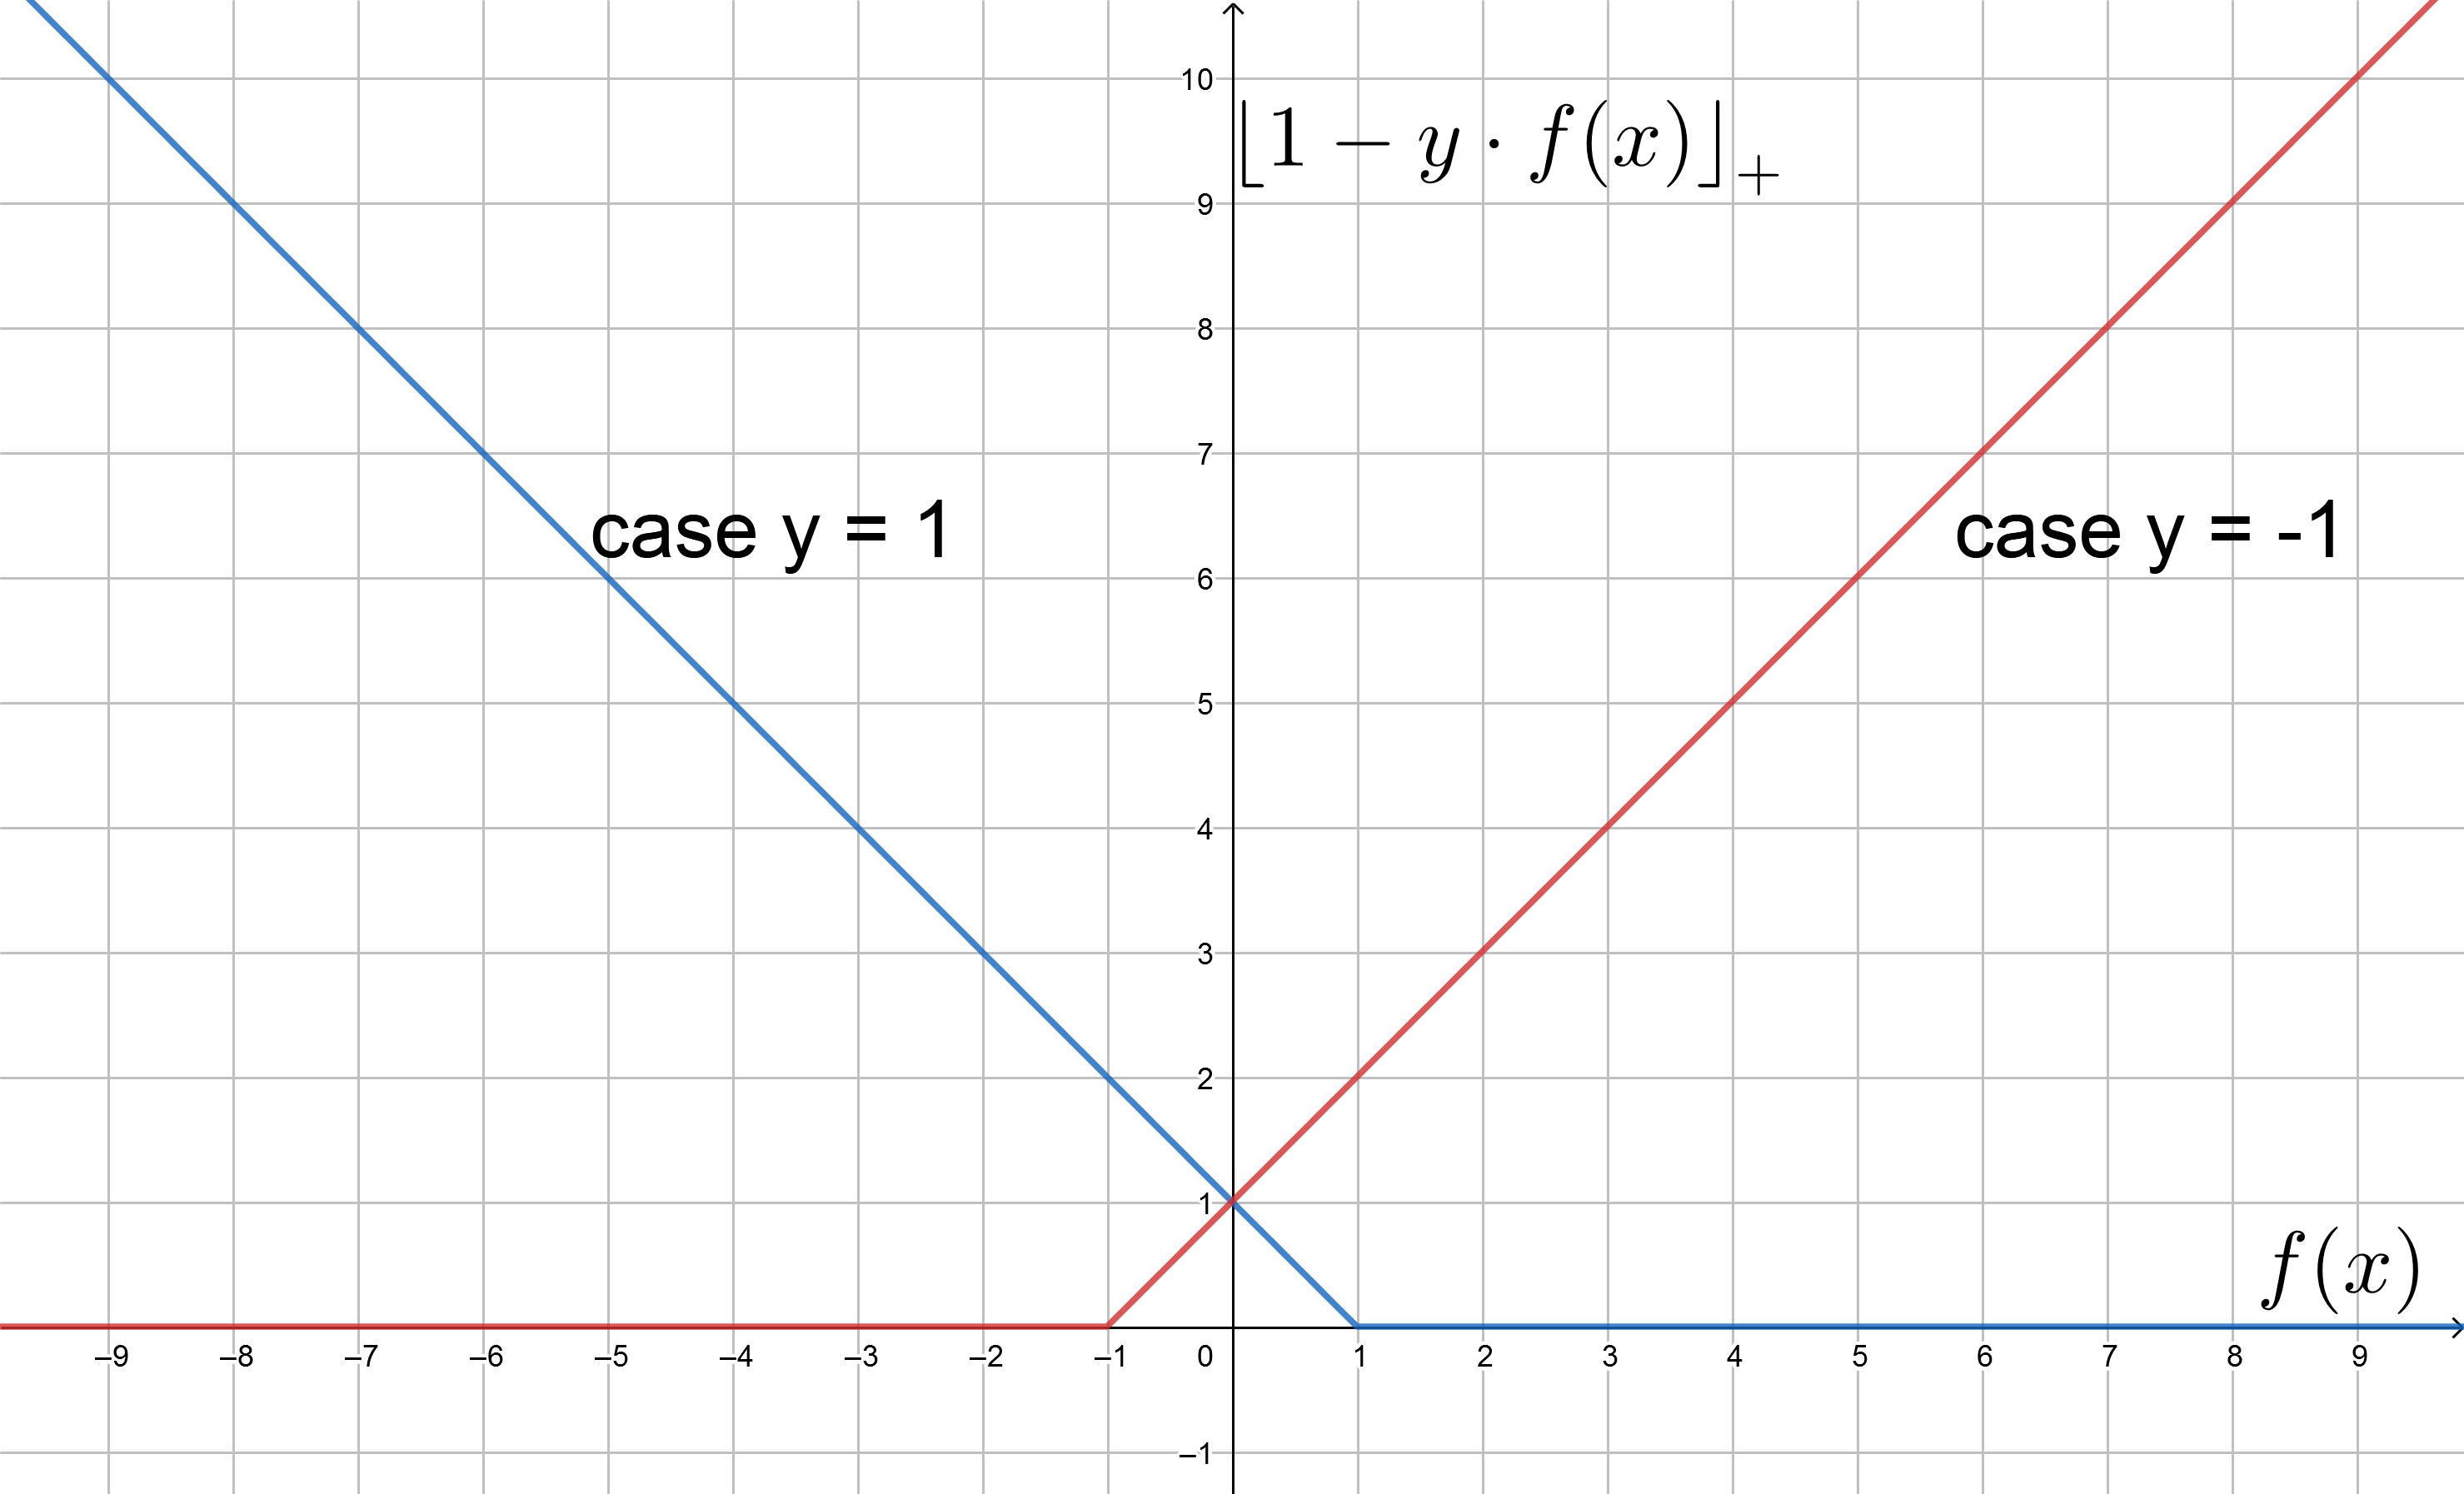
\includegraphics[width=0.7\linewidth]{images/svm-error.png}
 	\caption{%
 		الخطأ في العينة الواحدة في نموذج الـ \eng{SVM}.
 	}
 	\label{fig:svm:error}
 \end{figure}

يمكن البرهان على أنه في حالة كون المعطيات قابلة للفصل بخط مستقيم، فإن حل مسألة الأمثلة سيعطي المستقيم $f$ الذي يحقق أكبر هامش ممكن؛
أي اذا قمنا بحساب البعد بين كل نقطة وهذا المستقيم، فإن أصغر بعد سيكون أكبر ما يمكن، وهذا ما يوضحة الشكل~\ref{fig:svm:margin}.
 \begin{figure}[htb]
	\centering
	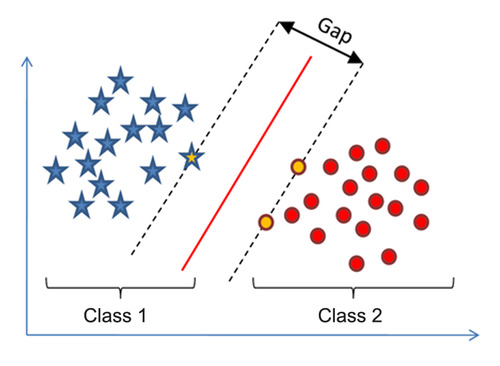
\includegraphics[width=0.5\linewidth]{images/svm-margin.jpg}
	\caption{
		مستقيم يفصل صفين بهامش أعظمي.
	}
	\label{fig:svm:margin}
\end{figure}

ولكن أيضاً يمكننا اختيار تابع غير خطي. هذا مفيد مثلاً في حال كان شكل مجموعة التدريب مثلما في الشكل~\ref{fig:svm:non-linear}.
 \begin{figure}[htb]
	\centering
	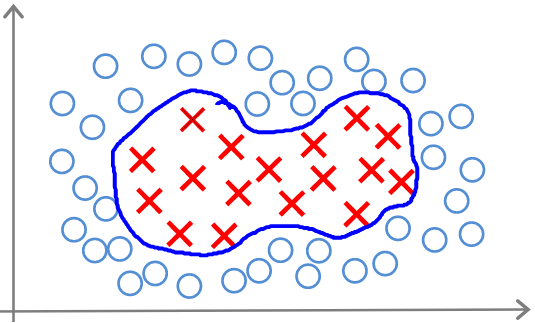
\includegraphics[width=0.5\linewidth]{images/svm-non-linear.PNG}
	\caption{
		مجموعة التدريب غير قابلة للفصل باستخدام مستقيم.
	}
	\label{fig:svm:non-linear}
\end{figure}
إذ يوجد أسلوب يسمى بالـ \eng{Kernel Trick}، يسمح لنا بفعل هذا.
ينص هذا الأسلوب على تعريف $f$ بالشكل
$ f(x) = \sum_{i=1}^{m} \theta_i K(x, x^{(i)}) + \theta_0 $%
، ثمّ حل مسألة الأمثلة السابقة ذاتها.
نلاحظ هنا أنه لدينا $ m+1 $ باراميتر عوض الـ $ n+1 $ باراميتر في الحالة السابقة.
و يسمى التابع $K$ بالنواة \eng{Kernel}.
فمثلاً اختيار
 $ K(u, v) = \sum_{j=1}^{n} u_j v_j $
يؤدي إلى حل مكافئ لحل المسألة الموضحة في المعادلة~\ref{eq:svm:primal}. تسمى هذه النواة بالنواة الخطية \eng{Linear Kernel}.
 
إنّ أشهر النوى المستخدمة عادةً هي:
\begin{doublespacing}
	\begin{center}
		\begin{tabular}{r l l}
			النواة الخطية & \eng{Linear Kernel} &
			 $ K(u, v) = u^T v $
			 \\
			 النواة الحدودية & \eng{Polynomial Kernel} &
			 $ K(u, v) = (u^T v + r)^d $
			 \\
			 النواة الغاوسية & \eng{Gaussian Kernel} &
			 $ K(u, v) = \exp{\left( -\gamma \norm{u - v}^2 \right)} $
		\end{tabular}
	\end{center}
\end{doublespacing}
إذ أن الرمز $u^T$ يرمز إلى المنقول وتحديداً فإن
$ u^T =
\left(\begin{smallmatrix}
u_1 \\ \vdots \\ u_n
\end{smallmatrix}\right)^T
= \left( u_1, \dots, u_n \right) $%
. تسمى النواة الغاوسية أيضاً بـ \eng{Radial Basis Function (RBF) Kernel}.
وننوه أن البارمترات المذكورة $ r, d, \gamma $ هي بارامترات فوقية.

لحل مسألة الأمثلة المطروحة، توجد العديد من الخوارزميات. هذا النوع من المسائل، ومسائل الأمثلة بشكل عام هو فرع
مدروس بشكل جيد في الرياضيات تحت اسم \eng{Mathematical Optimization}.
فتوجد العديد من الخوارزميات المستخدمة لحل مسألة الأمثلة المطروحة.
من أشهرها هي خوارزمية
\eng{Sequential Minimal Optimization (SMO)}%
. يتطلب شرحها الخوض في كثير من التفاصيل الرياضية وهو خارج نطاق هذا المشروع.


%آخر ما يجب ذكره، هو الأسلوب المستخدم للتصنيف في حال وجود أكثر من صفين.
%هذا الأسلوب مستخدم بشكل عام ويسمى بـ
%\eng{One-versus-One multi-class classification}%
%. الفكرة كالتالي، لأجل كل صفين، نعتبر جميع الصفوف الأخرى هي صف آخر.
%ونبني لكل صف، مُصنّف على هذا الأساس.
%الآن لأجل دخل جديد، نحسب $f$ لكل مُصنّف، ونأخذ الصف الذي يحقق أكبر قيمة.


آخر ما يجب ذكره، هو الأسلوب المستخدم للتصنيف في حال وجود أكثر من صفين.
فكما رأينا، إن خوارزمية الـ \eng{SVM} مبنية للتصنيف بين صفين فقط، وهذا ما يسمى بالتصنيف الثنائي \eng{binary classification}.
توجد عدّة أساليب تسمح باستخدام خوارزميات التصنيف الثنائي لإجراء تصنيف عندما يكون عدد الصفوف هو $ k > 2 $.
سنستخدم أسلوب يسمى بـ
\eng{One-versus-One multi-class classification}%
. الفكرة كالتالي، لأجل كل صفين مختلفين، نهمل بقيّة الصفوف، ونبني مصنّف للتمييز بين هذين الصفين.
أي نقوم ببناء $ k(k-1)/2 $ مصنف.
الآن لأجل عينة جديدة، نقوم بتطبيق هذه المصنفات جميعها، ونأخذ الصف الذي تم اختياره أكبر عدد من المرات.



\subsection{معايير التقييم}
\label{sec:metrics}
تختلف معايير تقييم صحة نماذج تعلم الآلة باختلاف نوع المسائل التي تقوم بحلها.
سنتحدث في هذه الفقرة عن أهم معايير التقييم المستخدمة في مسائل التصنيف.

بدايةً لنضع بعض الرموز لتبسيط العلاقات الرياضية وتوضيح الأفكار.
كما تحدثنا سابقاً عن مجموعة التدريب،
من المعتاد أن توجد معطيات أخرى مستقلة عن مجموعة التدريب تسمى بمجموعة الاختبار \eng{Test Set}.
حيث أنه بعد الحصول على النموذج الناتج من خوارزمية تعلم الآلة بتدريبه على مجموعة التدريب،
يتم اختبار هذا النموذج على مجموعة الاختبار.
سنرمز لها بـ \eng{TS}.
سنرمز لمجموعة عناصرها بـ $ (x_i, y_i) $، حيث $x_i$ هو شعاع السمات، $y_i$ هو الصف الموافق.
وسنرمز بـ $\hat{y}_i$ للصف الذي تنبأت به خوارزمية تعلم الآلة المستخدمة والتي نرييد تقييمها.
وسنستخدم الرمز $ \abs{\cdot} $ لعدد عناصر مجموعة ما.
فمثلاً إن $ \abs{y_i = c} $ هو عدد العناصر من \eng{TS} التي لها الصف $c$.

الصِحّة \eng{Accuracy} هي المعيار الأشهر. فهي نسبة العينات التي تم تصنيفها بشكل صحيح. أي:
$$ \mathrm{Accuracy} = \frac{ \abs{\hat{y}_i = y_i} }{ \abs{ \mathrm{TS} } } $$

إنّ هذا المعيار غير كافي للتعبير عن مدى قوة النموذج الناتج.
لنتأمل مثال تكون فيه مجموعة التدريب فيها صفين فقط.
نسبة ورود الصف الأول هو $1\%$،
مثل حالة تشخيص مرض نادر.
فبإمكاننا بسهولة الحصول على نموذج بدقة $99\%$.
هذا النموذج يتنبأ دائماً بالصف الثاني؛
فلكون ورود عينات تنتمي للصف الأول نادر جداً تكون صحة هذا النموذج عالية.
ولكن من الواضح أن هذا النموذج غير مجدي.
النقاش السابق يدفع لتحديد معايير أخرى للتقيم.

الدقّة \eng{Precision} هي معيار يعبر عن دقّة تصنيف صف معيّن.
دقّة تصنيف الصف $c$ هي نسبة العينات التي صنفت بشكل صحيح في الصف $c$ من بين جميع العينات التي صنفت بالصف $c$.
أي:
$$ \mathrm{Precision\ for\ class\ c} = \frac{ \abs{ \hat{y}_i = c \wedge y_i = c } }
{ \abs{ \hat{y}_i = c } } $$

الإرجاع \eng{Recall} هو معيار يعبر عن مدى استرجاعنا لعينات من صف معيّن.
معيار الإرجاع للصف $c$ هو نسبة العينات التي صنفت بشكل صحيح في الصف $c$ من بين جميع العينات التي هي ضمن الصف $c$ فعلاً.
أي:
$$ \mathrm{Recall\ for\ class\ c} =
\frac{ \abs{ \hat{y}_i = c \wedge y_i = c } }{ \abs{ y_i = c } } $$

المعيار الأخير الذي سنتحدث عنه يسمى بـ \eng{F1-score}.
ينتج من حاجتنا إلى الاعتماد على قيمة عددية واحدة فقط لمقارنة نموذجين معاً.
وهو معيار يجمع بين الدقّة والإرجاع.
النموذج المقترح للجمع بينهما هو:
$$ \mathrm{F1-score} = 2 \cdot \frac{ \mathrm{Precision} \cdot \mathrm{Recall}}
{\mathrm{Precision} + \mathrm{Recall}} $$
سنرمز لهذا المعيار اختصاراً بـ \eng{F-score}.
حيث أن الرقم $1$ في اسمه يدل على أننا نعطي للدقّة والإرجاع نفس الأهمية.
فهذا المعيار حالة خاصة من معيار أعم يسمح بإعطاء أهمية أكبر للدقّة على الإرجاع وبالعكس، ولكن لن نتحدث عنه.



\section{معالجة اللغات الطبيعية}
معالجة اللغات الطبيعية
\eng{Natural Language Processing (NLP)}
هو المجال الذي يدرس الآليات التي تسمح للحواسيب والآلات بفهم ومعالجة اللغات الطبيعية مثل اللغة العربية والإنكليزية وغيرهما~\cite{riad2017}.
ويعتبر مجال مهم في الذكاء الصنعي.
يتقاطع هذا المجال مع العديد من المجالات منها علم اللسانيات وتعلم الآلة وغيرهما.
سنتحدث في هذه الفقرة بشكل بسيط عن أهم المراحل في معالجة اللغات الطبيعية.

\begin{itemize}
	\item 

التحليل الصرفي \eng{Morphological Analysis} وهو المرحلة التي يجري فيها تحليل الكلمة إلى مكوناتها الأساسية.
يُنفّذ هذا التحليل على مستوى الكلمة دون النظر إلى السياق.
بشكل أساسي هناك مرحليتن لهذا التحليل. التقطيع \eng{Tokenization} والتجذير \eng{Stemming}.

خرج مرحلة التقطيع هو الرموز التي تكون الجملة \eng{Tokens}.
أي مثلاً إنّ الجملة \\
\centerline{ \eng{Google inc. is huge.} }
سيتم تقسيمها إلى خمس رموز وهي:\\
\centerline{ \eng{ \{Google | inc. | is | huge | .\} } }
لاحظ أن النقطة الأخيرة تعتبر رمز منفصل بينما النقطة في الكلمة \eng{inc.} ليست رمز منفصل.

خرج مرحلة التجذير هو جذر الكلمة، بالإضافة إلى السوابق واللواحق، ومعلومات أخرى تختلف باختلاف اللغة.
مثلاً إن جذر الكلمات
\eng{fish, fishing, fished, fisher}
هو \eng{fish}.
واللواحق هي
\eng{ing, ed, er}
على الترتيب.


\item
تحديد أنماط الكلمات \eng{Part-of-Speech Tagging} وهو عملية إسناد الأنماط النحوية الملائمة لكل كلمة من كلمات الجملة.
دخل هذه المرحلة عادةً يكون كلمة ضمن سياق محدد (ضمن جملة).
الخرج الناتج يكون النمط النحوي لهذه الكلمة (اسم، فعل، صفة، إلخ).

\item
التقطيع الجمل \eng{Chunking} وهو تقسيم الجملة إلى عبارات أصغر؛ أي عبارات اسمية، أو عبارات فعلية، إلخ.
يوضح الشكل~\ref{fig:nlp:chunking} مثال على ذلك.

 \begin{figure}[htb]
	\centering
	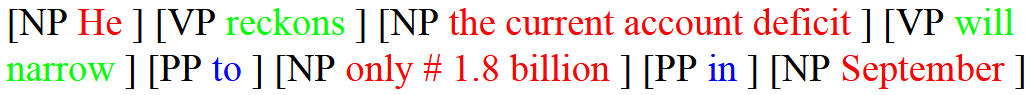
\includegraphics[width=0.7\linewidth]{images/nlp-chunking2.PNG}
	\caption[%
		مثال عن عملية التقطيع الجمل.
	]{%
		عمليّة التقطيع الجمل للجملة
		\eng{He reckons the current account deficit will narrow to only \# 1.8 billion in September}%
%		\eng{He reckons the current account deficit will narrow to only \#}%
		. تم تقسيم هذه الجملة إلى جمل فعلية
		\eng{Verb Phrase (VP)}%
		، وجمل اسمية
		\eng{Noun Phrase (NP)}%
		، وعبارات جر
		\eng{Prepositional Phrase (PP)}.
	}
	\label{fig:nlp:chunking}
\end{figure}

\item
الشجرة النحوية \eng{Parsing Tree}.
في الواقع يمكن اعتبار الشجرة النحوية الخرج الناتج عن العمليات السابقة مجتمعة.
حيث يتم تمثيل الجملة كشجرة.
انظر الشكل~\ref{fig:nlp:tree} لمثال توضيحي.
الاختصارات المكتوبة،
مثل \eng{NN} تعني اسم مفرد \eng{singular noun}،
\eng{NNS}
تعني اسم جمع \eng{plural noun}.
وللإطلاع على هذه القائمة كاملةً انظر~\cite{penntreebank}.


 \begin{figure}[htb]
	\centering
	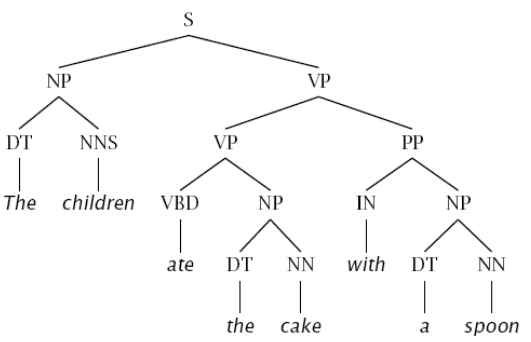
\includegraphics[width=0.7\linewidth]{images/nlp-tree.PNG}
	\caption[%
		مثال عن الشجرة النحوية.
	]{%
		الشجرة النحوية الناتجة للجملة
		\eng{The children ate the cake with a spoon}.
	}
	\label{fig:nlp:tree}
\end{figure}

\item 
تحليل التّبعية \eng{Dependency Parsing}.
نظراً لقصور الشجرة النحوية عن إعطاء كامل المعلومات حول الجملة المدروسة،
تم اقتراح تمثيل المعلومات النحوية على شكل بيان التبعية \eng{Dependency Graph}.
يوضح هذا البيان العلاقات النحوية بين كلمات الجملة.
إذ يتكون من عقد تمثّل الكلمات ووصلات تحدد العلاقة بين هذه الكلمات.
يبيّن الشكل~\ref{fig:nlp:graph} مثالاً على خرج تحليل التبعية.
الاختصارات المكتوبة للعقد هي ذاتها المستخدمة في حالة الشجرة النحوية.
الاختصارات المكتوبة للوصلات،
مثل \eng{det} تربط بين الاسم وأداة التعريف المرتبطة به،
\eng{nsubj}
تربط بين الفعل والفاعل.
وللإطلاع على هذه القائمة كاملةً انظر~\cite{dependency-graph}.

 \begin{figure}[htb]
	\centering
	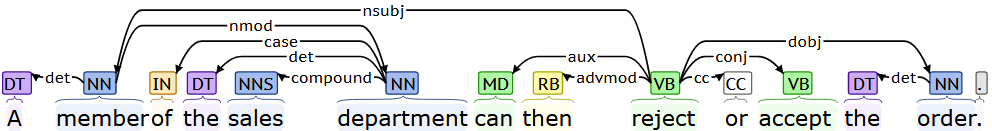
\includegraphics[width=0.85\linewidth]{images/nlp-graph.PNG}
	\caption[%
		مثال عن بيان التبعية.
	]{%
		بيان التبعية الناتج للجملة 
		\eng{A member of the sales department can then reject or accept the order.}.
	}
	\label{fig:nlp:graph}
\end{figure}

\item 
حل الغموض في حالات الإحالة \eng{Anaphora Resolution}.
الإحالة \eng{Anaphora} هي استخدام ضمائر أو تعابير للإشارة إلى اسم أو تعبير تم ذكره في سياق سابق في النص.
فإذا تأملنا المثال التالي: \\
\centerline{\eng{ \textbf{They} buy the \underline{issue}, then resell \underline{it} to the public.}}
إن \eng{it} تشير إلى \eng{issue}.
وفي هذه الحالة يكون المشار إليه واقعاً في نفس الجملة.
أمّا في حالة \eng{They} فيكون المشار إليه واقعاً في جملة سابقة.

\end{itemize}



\section{أهم الأبحاث المشابهة}
كما شرحنا في الفقرة~\ref{sec:ml} وتحديداً الفقرة~\ref{sec:ml:steps}، إن أولى الخطوات اللازمة لتنجيز أي نظام يستخدم تعلم الآلة
هي تحديد السمات التي سيتم استخدامها.
فهذا المشروع يتعامل مع النصوص وكون المسألة المطروحة هي تقييم جودة هذه النصوص من ناحية سهولة القراءة،
فمن المهم جداً معرفة السمات التي ستعبّر عن وتوصّف جودة نص.

بالعودة إلى العديد من الأوراق العلمية التي تتقاطع مع هذا المشروع،
تم تجميع عدد من الأفكار والمنهجيات التي تم تبنيها والاعتماد عليها كإطار عمل ضمن المشروع.
سنذكر في هذه الفقرة أهم الأوراق العلمية التي تمت دراستها،
وأهم الأفكار والمنهجيات المتبعة فيها.
بالإضافة إلى السمات وخوارزميات تعلم الآلة المستخدمة لحل مسائل مشابهة للمسألة المطروحة في هذا المشروع.

إن فكرة تقييم النصوص من ناحية صعوبة القراءة بشكل موضوعي (غير شخصي) بدأت تقريباً منذ قرن.
الأفكار الأولية التي واجهت هذا الموضوع هي عبارة عن علاقات رياضية بسيطة.
ولقد اعتَمَدَت على خصائص سطحية في النص المدروس.
مثل متوسط طول الجملة، ومتوسط طول الكلمة.
فمثلاً إن \eng{Flesch Score} يعطى بالعلاقة
$$ \mathrm{Flesch\ Score} = 206.835 -
1.015 \cdot \frac{\mathrm{\# words}}{\mathrm{\# sentences}}
- 84.6 \cdot \frac{\mathrm{\# syllables}}{\mathrm{\# words}} $$
أي يمثل علاقة خطية لمتوسط طول الجملة بالكلمات، ومتوسط طول الكلمة بالمقاطع الصوتية.
وكلما كان هذا المقدار أكبر، كلما كان النص أسهل للقراءة.
في~\cite{dubay2007} أُجريب مقارنة بين عدد واسع من هذه العلاقات.
وفي~\cite{readability-scores-gutenberg} تم رسم ودراسة توزع عدد من هذه المعايير على عدد كبير من النصوص.
على الرغم من كون هذه العلاقات تبدو سطحية من ناحية التمثيل اللغوي للنص،
تم اعتمادها بشكل واسع لمدة من الزمن.

كما ظهرت نماذج أكثر تعقيداً تعتمد على مفهوم الـ \eng{n-gram}.
وهو نموذج إحصائي لتمثيل اللغة؛ يعبر عن احتمال ورود كلمة ضمن سياق معيّن، أو احتمال ورود جملة أو سياق معيّن.
وهو تمثيل بسيط للانتروبية في اللغة الانكليزية.
استخدم هذا المفهوم بالإضافة إلى سمات أخرى بُنيت فوقه ومستوحاة من مفهوم الانتروبية في عدد من الدراسات
أهمها~\cite{schwarm2005, petersen2009}.
وكانت النتائج أفضل بشكل واضح عن نتائج المعايير السابقة والمعتمدة على علاقات رياضية بسيطة.
حيث تم الاعتماد على خوارزميات تعلم الآلة.
الخوارزمية الأكثر استخداماً والتي حققت أفضل النتائج كانت الـ \eng{SVM}.

مع تطور الأدوات في معالجة اللغات الطبيعية، أصبح من الممكن أن نأخذ بعين الاعتبار مؤشرات أقوى، مفرداتية ونحوية وغيرها.
في~\cite{feng-phd, feng2010comparison} تمت دراسة ومقارنة العديد من السمات
التي تعتمد بشكل أساسي على تقدم الأدوات في معالجة اللغات الطبيعية.
حيث تمت مقارنة عدّة سمات، وبعدّة أنواع.
مثل التنوع في الأفعال، والكلمات المستخدمة، وكثافة الأسماء المستخدمة في النص.
بالإضافة إلى الترابط بين الجمل باستخدام بيان التبعية والعديد غيرها.
أفضل نتيجة تم تحقيقها كانت باستخدام الـ \eng{SVM} على مجموعة جزئية من السمات المدروسة.

أيضاً لقد تمت دراسة تعقيد النصوص المكتوبة من قبل الطلاب الذين يتعلمون اللغة الانكليزية.
تم ذلك تحت ما يسمى أبحاث تعلم اللغات \eng{second language acquisition}.
حيث تمت دراسة عدد من المؤشرات التي تعبر عن تعقيد النص، بما يفيد في دراسة تحسن الطلاب أثناء تعلمهم للغة.
كما أن دراسات لاحقة قامت بأتمتت آليات حساب هذه المؤشرات أهمها~\cite{lu2010}.
فكان تغيير هذه المؤشرات مع الزمن، يبيّن مستوى تحسن الطلاب في تعلم اللغة.
وكان أول استخدام لهذه الدراسات لبناء نموذج تعلم آلة لتقييم جودة النصوص هو في~\cite{vajjala2012}.
حيث تم الاعتماد على سمات مستوحاة بشكل مباشر من هذه المؤشرات.
معظم هذه السمات تعبر عن تعقيد تراكيب الجمل.
مثل وجود جمل شرطية أو جمل معطوفة على بعضها وهكذا.

أيضاً تم استخدام سمات تعبر عن نسبة ورود كلمات معينة ضمن النص.
فإن ورود كلمات متقدمة ضمن النص وبتواتر عالي قد يكون مؤشر جيد على كون النص بمستوى متقدم.
هذه الكلمات تكون غالباً منتقاة من مصدر تعليمي.
فقد تم استخدام كلمات من المصدر
\eng{The Academic Word List%
	\footnote{
		للإطلاع على هذه القائمة كاملةً انظر~\cite{academic-word-list}.
	}
}
في~\cite{vajjala2012,vajjala2014,vajjala2018}.
و تم استخدام كلمات من المصدر
\eng{English Vocabulary Profile%
	\footnote{
		لمزيد من التفاصيل انظر
		\url{http://www.englishprofile.org}.
	}
}
في~\cite{xia2016}.
حيث تبيّن أن لهذه السمات دور جيد في تحسين أداء النماذج الناتجة.

سنوضح لاحقاً  وبتفصيل أكبر في الفقرة~\ref{sec:sys:features} السمات المستخدمة في هذا المشروع.
يجب أيضاً التنويه إلى المعطيات المستخدمة في هذه الدراسات.
إن معظم المعطيات هي من مصدر تعليمي،
مثل مجلات تعليمية للأطفال حيث أن المقالات مصنفة بحسب الفئة العمرية المناسبة.
سنتحدث لاحقاً في الفقرة~\ref{sec:sys:datasets} عن مجموعة المعطيات المستخدمة في هذا المشروع وخصائصها.



